\documentclass[
	% -- memoir class options --
	12pt,	% font size
	openright, % chapters begin on odd pages only (inserts blank page if needeed)
	oneside, % or twoside
	a4paper, % paper size
	% -- abntex2 class options --
	%chapter=TITLE, % uppercase chapter titles
	%section=TITLE, % uppercase section titles
	%subsection=TITLE, % upptercase subsection titles
	%subsubsection=TITLE,% idem
	% -- babel package options --
	% french, % aditional language for hyphenation
	% spanish, % aditional language for hyphenation
	brazil, % aditional language for hyphenation
	english % the last language is the main one
]{abntex2}

% ----------------------------------------------------------
% BASIC PACKAGES
\usepackage{lmodern} % Font Latin Modern
\usepackage[T1]{fontenc} % Source code selection
\usepackage[utf8]{inputenc} % Use UTF-8
\usepackage{lastpage} % Used by the catalographic-card
\usepackage{indentfirst} % Paragraph identation
\usepackage{color} % Color control
\usepackage{graphicx} % Include charts
\usepackage{microtype} % Justification improvements
\usepackage{listings} % Source code insertion
\usepackage{nomencl} % Used for indexing
\usepackage{babelbib}

% Quotation packages
\usepackage[brazilian,hyperpageref]{backref} % References quotations
\usepackage[alf]{abntex2cite} % ABNT default quotations

% PACKAGES CONFIGURATIONS
% backref
\renewcommand{\backrefpagesname}{Quoted in page(s):~}
% Text before page numbers
\renewcommand{\backref}{}
% Quotation texts
\renewcommand*{\backrefalt}[4]{
  \ifcase #1 %
      No quotations in text.%
  \or
      Quoted in page #2.%
  \else
      Quoted #1 times in pages #2.%
  \fi
}

\usepackage{lipsum} % Dummy text generation

% ENGLISH TRANSLATION
\newcommand{\institution}{\instituicao}
\newcommand{\printinstitution}{\imprimirinstituicao}

\newcommand{\advisor}{\orientador}
\newcommand{\printadvisor}{\imprimirorientador}
\newcommand{\printadvisorLabel}{\imprimirorientadorRotulo}

\newcommand{\typeofdocument}{\tipotrabalho}
\newcommand{\printtypeofdocument}{\imprimirtipotrabalho}

\newcommand{\preamble}{\preambulo}
\newcommand{\printpreamble}{\imprimirpreambulo}

\newcommand{\coadvisor}{\coorientador}

\newcommand{\printcover}{\imprimircapa}

\newcommand{\printlocal}{\imprimirlocal}

\newcommand{\printcoversheet}{\imprimirfolhaderosto}

\newcommand{\printtitle}{\imprimirtitulo}

\newcommand{\printdate}{\imprimirdata}

\newcommand{\printauthor}{\imprimirautor}

\newcommand{\signature}{\assinatura}

\newenvironment{catalographiccard}{\fichacatalografica}{\endfichacatalografica}
\newenvironment{approvalsheet}{\folhadeaprovacao}{\endfolhadeaprovacao}
\newenvironment{dedication}{\dedicatoria}{\enddedicatoria}
\newenvironment{acknowledgements}{\agradecimentos}{\endagradecimentos}
\newenvironment{inscription}{\epigrafe}{\endepigrafe}
\newenvironment{summary}{\resumo}{\endresumo}
\newenvironment{acronyms}{\siglas}{\endsiglas}
\newenvironment{listofsymbols}{\simbolos}{\endsimbolos}
 % Translate abntex macros to english
% Just use the next file to tranlate any portuguese word in the bibliography
\bibliographystyle{configurations/english-abntex-cite} % Translate bibliography
 % PACKAGES
% ----------------------------------------------------------

% ----------------------------------------------------------
\title{Guitar Digitizer}
\author{Cristóvão Diniz Trevisan \and Viktor Volochtchuk}
\local{Brazil}
\date{2017, v-0.0.1}
\advisor{Gustavo Benvenutti Borba}
% \coadvisor{Equipe \abnTeX}
\institution{%
  Federal University of Technology - Paraná -- UTFPR
  \par
  Electronic Engineering
  \par
  Graduation Program}
\typeofdocument{Graduation Final Project}
\preamble{Project presented as graduation material for the course of Electronic
Engineering at UTFPR}
 % COVER AND COVER SHEET
% ----------------------------------------------------------

% ------------------------------------------------------------------------
% CONFIGURATIONS
% ------------------------------------------------------------------------

% changing blue color appearance
\definecolor{blue}{RGB}{41,5,195}

% pdf file information
\makeatletter
\hypersetup{
	% pagebackref=true,
	pdftitle={\@title},
	pdfauthor={\@author},
	pdfsubject={\printpreamble},
	pdfcreator={LaTeX with abnTeX2},
	pdfkeywords={guitar}{digitizer}{MIDI}{pitch}{detection}{hexaphonic},
	colorlinks=true, % false: boxed links; true: colored links
	linkcolor=blue, % color of internal links
	citecolor=blue, % color of links to bibliography
	filecolor=magenta, % color of file links
	urlcolor=blue,
	bookmarksdepth=4
}
\makeatother

% Spacing between lines and paragraphs
\setlength{\parindent}{1.3cm}

% Spacing between paragraphs
\setlength{\parskip}{0.2cm}  % also try \onelineskip

% compiles the index
\makeindex
\makenomenclature

% ----------------------------------------------------------
\begin{document} % BEGIN DOCUMENT
% ----------------------------------------------------------

% Remove the obsolete space between lines
\frenchspacing

% ------------------------------------------------------------------------------
\pretextual % PRE TEXTUAL ELEMENTS
% ------------------------------------------------------------------------------

% cover
\printcover

% coversheet
% (* teels to build a bibliographic record)
\printcoversheet*

% This is an example to be replaced with the actual catalographic card (using the macro bellow)
% \begin{catalographiccard}
%     \includepdf{catalographiccard.pdf}
% \end{fichacatalografica}
\begin{catalographiccard}
	\vspace*{\fill}					% Posição vertical
	\hrule							% Linha horizontal
	\begin{center}					% Minipage Centralizado
	\begin{minipage}[c]{12.5cm}		% Largura

	\printauthor

	\hspace{0.5cm} \printtitle  / \printauthor. --
	\printlocal, \printdate-

	\hspace{0.5cm} \pageref{LastPage} p. : il.\\

	\hspace{0.5cm} \printadvisorLabel~\printadvisor\\

	\hspace{0.5cm}
	\parbox[t]{\textwidth}{\printtypeofdocument~--~\printinstitution,
	\printdate.}\\

	\hspace{0.5cm}
		1. Hexaphonic Guitar
		2. Digitizer
		3. MIDI
		4. Pitch Detection
		I. Guitar Digitizer
		II. \printadvisor
		III. Federal University of Technology - Paraná
		IV. Electronic Engineering\\

	\hspace{8.75cm} CDU 02:141:005.7\\

	\end{minipage}
	\end{center}
	\hrule
\end{catalographiccard}

% % ---------------     NOT USED     ----------------
\begin{errata}
Elemento opcional da \citeonline[4.2.1.2]{NBR14724:2011}. Exemplo:

\vspace{\onelineskip}

FERRIGNO, C. R. A. \textbf{Tratamento de neoplasias ósseas apendiculares com
reimplantação de enxerto ósseo autólogo autoclavado associado ao plasma
rico em plaquetas}: estudo crítico na cirurgia de preservação de membro em
cães. 2011. 128 f. Tese (Livre-Docência) - Faculdade de Medicina Veterinária e
Zootecnia, Universidade de São Paulo, São Paulo, 2011.

\begin{table}[htb]
\center
\footnotesize
\begin{tabular}{|p{1.4cm}|p{1cm}|p{3cm}|p{3cm}|}
  \hline
   \textbf{Folha} & \textbf{Linha}  & \textbf{Onde se lê}  & \textbf{Leia-se}  \\
    \hline
    1 & 10 & auto-conclavo & autoconclavo\\
   \hline
\end{tabular}
\end{table}

\end{errata}

% This is an example to be replaced with the actual approvation sheet (using the macro bellow)
% \includepdf{approval-sheet.pdf}
%
\begin{approvalsheet}

	\begin{center}
		\begin{center}
			\MakeUppercase{\printauthorone} \\
			\MakeUppercase{\printauthortwo} \\
		\end{center}

		\vspace*{\fill}\vspace*{\fill}
		\begin{center}
			\Large
			\MakeUppercase{
				\imprimirtitulo
			}
		\end{center}
		\vspace*{\fill}
	\end{center}

	\noindent
	This final year project report was presented in February 15, 2018 to the Department of
	Electronics's (DAELN) of the Federal University of Technology - Paraná (UTFPR), in
	partial fulfillment of the requirements for the degree of Electronics Engineer.
	The work was approved by the committee members bellow.
	\vspace*{\fill}

	\noindent
	\textit{
		Este relatório de trabalho de conclusão de curso foi apresentado em 15 de fevereiro
		de 2018 ao Departamento Acadêmico de Eletrônica (DAELN) da Universidade Tecnológica
		Federal do Paraná (UTFPR) como requisito parcial para obtenção do título de Engenheiro
		Eletrônico. O trabalho foi aprovado pela banca examinadora composta pelos membros abaixo.
	}

	\vspace*{\fill}
	\vspace*{\fill}

	\signature{\textbf{Prof. Dr. Gustavo Borba \\ (DAELN - UTFPR)} \\ Advisor}
	\signature{\textbf{Mikhail Anatholy Koslowski \\ (Engineer at Pumatronix - Curitiba)} \\ Co-advisor}
	\signature{\textbf{Prof. M.Sc. Leonardo Gomes Tavares \\ (Universidade Positivo - UP)}}
	\signature{\textbf{Prof. M.Sc. Ricardo Pedroni \\ (DAELN - UTFPR)}}

  \vspace*{\fill}
\end{approvalsheet}

\begin{dedication}
   \vspace*{\fill}
   \centering
   \noindent
   \textit{ This work is dedicated to those who supported our way through
   engineering course, even more when ourselves tried to give up. } \vspace*{\fill}
\end{dedication}

\begin{acknowledgements}

We give our special thanks to Eng. Mikhail Anatholy Koslowski, who gave us both
intellectual (since he once used an equipament with the same purposed) and
physical support (with compenents importation and equipaments).
Also to our advisor \advisor, who was present even in the moment that the initial
idea came to life, in a situation nobody else would have stayed.

\end{acknowledgements}

% \begin{inscription}
    \vspace*{\fill}
	\begin{flushright}
		\textit{``Não vos amoldeis às estruturas deste mundo, \\
		mas transformai-vos pela renovação da mente, \\
		a fim de distinguir qual é a vontade de Deus: \\
		o que é bom, o que Lhe é agradável, o que é perfeito.\\
		(Bíblia Sagrada, Romanos 12, 2)}
	\end{flushright}
\end{inscription}

\setlength{\absparsep}{18pt} % adjust the spacing of paragraphs

% summary in english
\begin{summary}[Abstract]
  Guitar are one of most popular instruments today, but there is one big disadvantage
  to use it: there is no good and affordable way to digitalize it's music. The
  biggest problem with this is the cost to annotate music, as it needs to be done
  by manually. This project tries to build one such system, building from passive
  hardware (hexaphonic pickup) to modern signal processing (pitch detection),
  attempting to produce a cheap and effective equipment for guitar music annotation
  by means of generating MIDI format data.


  \textbf{Key-words}: guitar. digitizer. MIDI. pitch. detection. hexaphonic.
\end{summary}

% summary in portuguese
\begin{summary}[Resumo]
  \begin{otherlanguage*}{portuguese}
    Violões e guitarras estão entre os instrumentos mais populares da atualidade,
    mas existe uma grande desvantagem em os utilizar: não há um meio barato e eficaz
    para digitalizar sua música. O grande problema com isso é o alto custo para
    transcrever partituras, que atualmente é um processo manual. Esse projeto tenta
    construir um sistema com esse propósito, criando desde sensores passivos (captador
    hexafônico) até processamento digital de sinais moderno (detecção de nota),
    visando um produto barato e eficaz para anotação musical através da geração de
    dados no format MIDI.

    \textbf{Key-words}: guitarra. digitalizador. MIDI. nota. detecção. hexafônico.
  \end{otherlanguage*}

\end{summary}

% ----------------------------- NOT COMPILED -----------------------------------
% % summary in french
% \begin{summary}[Résumé]
%  \begin{otherlanguage*}{french}
%     Il s'agit d'un résumé en français.
%
%    \textbf{Mots-clés}: latex. abntex. publication de textes.
%  \end{otherlanguage*}
% \end{summary}
%
% % summary in spanish
% \begin{summary}[summaryn]
%  \begin{otherlanguage*}{spanish}
%    Este es el summaryn en español.
%
%    \textbf{Palabras clave}: latex. abntex. publicación de textos.
%  \end{otherlanguage*}
% \end{summary}


% list of figures
\pdfbookmark[0]{\listfigurename}{lof}
\listoffigures*
\cleardoublepage

% list of tables
\pdfbookmark[0]{\listtablename}{lot}
\listoftables*
\cleardoublepage

\begin{acronyms}
  \item[MIDI] Musical Instrument Digital Interface
  \item[UI] User Interface
  \item[GUI] Graphical User Interface
  \item[API] Application Programming Interface
  \item[USB] Universal Serial Bus
  \item[DOM] Document Object Model
  \item[n.d.] No Date
\end{acronyms}


\begin{listofsymbols}
  \item[$ \Omega $] Ohm resistance unit
\end{listofsymbols}


% Summary
\pdfbookmark[0]{\contentsname}{toc}
\tableofcontents*
\cleardoublepage

% ------------------------------------------------------------------------------
\textual % TEXTUAL ELEMENTS
% ------------------------------------------------------------------------------

\chapter[Introduction]{Introduction}

With the advance of technology, music - and musical instruments - have also evolved to
use it's advantages. They are a lot of use cases, the most noticeable ones being music
annotation and creation (through electronic instruments, also known as synthesizers).
All of the modern musical software and hardware use the same format to communicate,
called MIDI. \\
To translate music playing it is needed to know which note is being played at a
given time. This make it very easy to translate instruments that have separated
keys for each note (the most noticeable one being piano) to MIDI, but very hard
do the same for instruments like the guitar, that have a single output for multiple
notes (each string has about 15 notes). The guitar is also a harmonic instrument,
as it can play multiple notes simultaneously, which makes it's digitization even harder.\\
There are already a few commercial solutions for this, but not a very performant
and cheap one. Recently a new pure software solution was released at a reasonable
price which works very well for live MIDI playing, but not enough for music annotation.
There are also a few hardware solutions available at the market, which perform well,
but are very expensive. \autoref{market-solutions} shows the most relevant solutions
in the current market.

\begin{table}[htb]
  \begin{center}
    \ABNTEXreducedfont
    \caption[Market Solutions]{Market Solutions}
    \label{market-solutions}
    \begin{tabular}{m{4cm} | m{1cm} | m{2cm} | m{2cm} | m{2cm} }
      \hline
      Name & Price (U\$D) & \pbox{2cm}{Usage\\Complexity} & \pbox{2cm}{Live\\Performance} & \pbox{2cm}{Annotation\\Performance}\\
      \hline \hline
      Roland GK3 + GhostHexpander + GI20 & 700 & Hard & High & High \\
      Godin Freeway + GhostHexpander + GI20 & 800 & Hard & High & High \\
      Jam Origin - Audio to MIDI & 100 & Easy & High & Low/Medium \\
      Migic & 40 & Easy & Medium & Low \\
      \hline
    \end{tabular}
    \legend{Source: authors}
  \end{center}
\end{table}

TODO: cost analysis

\section{Social Motivation}
Guitar music annotation is very expensive as of today. The reason for this is that
it takes a lot of effort to write a music sheet. In the way to make music annotation
cheaper and more accessible this project also aim to do this kind of work in a cheap
and easy way (that does not even require the knowledge of music annotation). \\
This would create great social meaning as it makes possible for everyone that play
the guitar to quickly write down their own compositions and arrangements and thus
share their culture to the world. \\
In specific this project was thought for the people that make their own arrangements
but don't share it because of the great time cost involved, most of them being YouTube
guitar players all over the world. The few that do share their annotations today usually
charge for it, thus blocking culture sharing. \\

\section{Foremost Project Decisions}
There are many ways to accomplish this objective, a few considered were through
mechanical pressure detection, pure software (like the commercial solutions) and
finally electromagnetic fields. \\
Mechanical pressure (or buttons) was discarded because it is still needs to detect
string vibration, which requires electromagnetic detection (to be cheap). But the latter can
be used as the only input, so it does not make sense to use both. \\
Software only detection is too hard to implement and does not guarantee good results.
This approach is still being developed now days by using the most recent advanced
techniques of machine learning. This is so state of the art that requires a really high
amount of money and effort to accomplish, which is not compatible to our resources
(as we are mere undergrad students). \\
Electromagnetic detection is nothing new (it is the base principle of electric guitars).
The only unusual approach we need is to get a separated signal for each string, thus
removing most of the software complexity quoted above, because we can them deal
with monophonic signals (as each string can only play one note at a time). It is
still complex to build a project with this decision, but it is feasible, and so
the chosen option.

\section{Electromagnetic Field Detection Approach Considerations}
TODO: explain high level architectural decisions, with flow diagram from: \\
passive hardware  -> active hardware -> firmware -> software (divided by parts)

\part{Hardware}

% TODO: include chapters, ex.:
% \input{textual-elements/hardware/part-x}}

\chapter{Hardware}
\section{Initial Idea}
The project started with the idea of assembly a system which should capture de guitar sound and change the sound to any another instrument. The system should be competitive with other existent devices.\\
To reach this objective it was verified the features which the project should reach and the methods necessaries to perform the desired actions.\\
\section{Pickup Project} 
After some studies it was decided to assembly a hexaphonic pickup instead buy one already manufactured, which is an expansive device. To reduce the cost of the project it was projected and printed the pickup base on 3D printer as the project showed on figure 1.

\begin{figure}[!htpb]
\centering
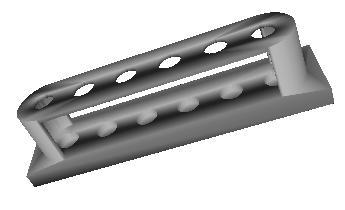
\includegraphics[scale=0.5]{textual-elements/hardware/Capt}
\caption{Pickup Base}
\end{figure}

After print the pickup base it was assembled the coils, composed by guitar magnets and copper iron (150 revolutions for each magnet), responsible for the transformation of the mechanic vibration of the string to the electric signal which is needed.   

\begin{figure}[!htpb]
\centering
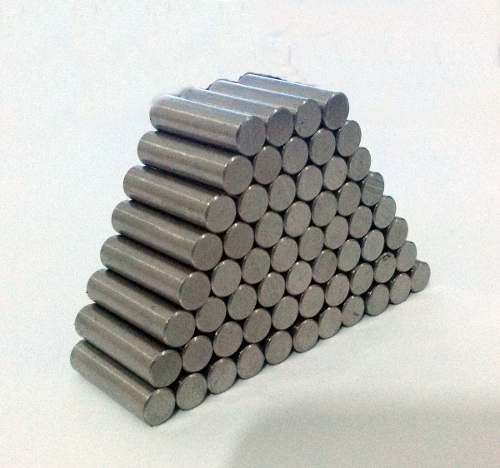
\includegraphics[scale=0.3]{textual-elements/hardware/ima}
\caption{Magnets}
\end{figure}

With the pickup already assembled it was verified the output signal. This signal pick was about 0.5 mV and ths value was so weak to send to the Analogic-digital converter present on the microprocessor. With this dungeon it was verified that it is needed a circuit responsible for the signal amplification to be possible to read the signal with quality on the microprocessor. 

\section{Amplifier Circuits}
It was researched some types of amplifiers circuits, it was selected the circuits with single supply, because the project was designed to be the maximum embedded on the guitar, without the needing of other supplies except the guitar battery or the USB connection of the microprocessor.
After some researches it was decided try two circuit types, with two different operational amplifiers. The first circuit uses the Texas Instruments INA 326 Instrumental Amplifier and the second uses the Texa Instruments TLV 4316 Operational Amplifier.

\subsection{INA 326}
The project using the INA 326 IC, started with a research at the datasheet of this compnent and it was verified one circuit which provides the desired Gain to the electric signal from the pickup respecting the project's initial requests. The circuit is shown on figure 3. 

\begin{figure}[!htpb]
\centering
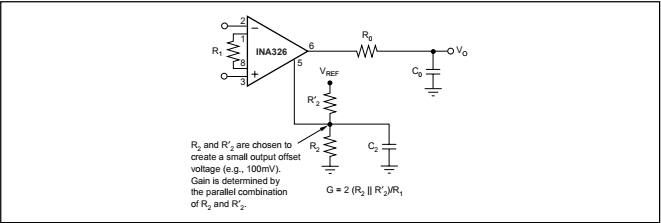
\includegraphics[scale=0.8]{textual-elements/hardware/Texas}
\caption{Amplifier assembly}
\end{figure}

This circuit amplifies the signal and the gain is obtained by the following equation:

$$G=2*\frac{(R_2||R_2 ')}{R_1}$$

On the project the Resistor $R_0$ and the Capacitor $C_0$ was excluded because it was not relevant on the output to this project. After the research it was developed a schematic model to perform some simulation tests to verify and prove the functionalism of the circuit for the desired application. The schematic circuit it was developed using the software CadSoft Eagle Professional 7.6.0 until the version showed at figure 4.

\begin{figure}[!htpb]
\centering
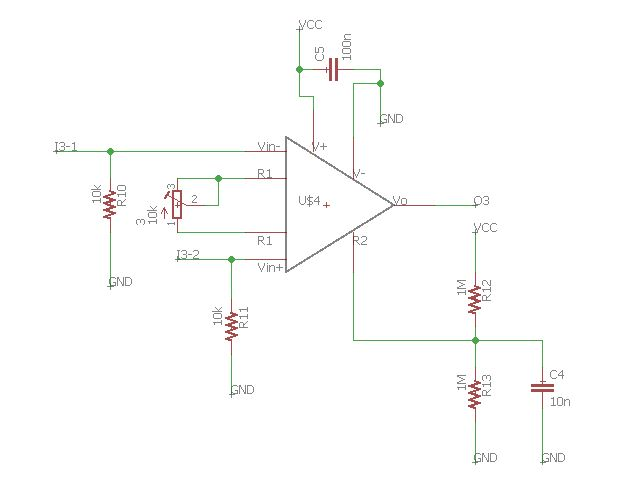
\includegraphics[scale=0.7]{textual-elements/hardware/INA}
\caption{Schematic for each channel}
\end{figure}

This circuit as showed on the image provides a Gain of:

$$G=2*\frac{(1M\Omega||1M\Omega)}{10k\Omega}$$
$$G=2*\frac{500k\Omega}{10k\Omega}$$
$$G=2*50$$
$$G=100$$

The amplifier circuit was projected to each channel. So the circuit needed 6 IC INA 326 to be complete. The complete schematic is showed on annex 1. After project the schematic circuit to each channel it was developed the PCB project, using the same software described on the schematic modelling. The PCI project is showed on figure 5.\\

This PCB project was projected on a dual layer board scheme, using 15 mils of minimum width for the conductive tracks. It was assembled on FR4 dual layer copper board, combining the through-hole and surface-mount technologies. This choice was made due the facility of the assembly of the through-hole components. It was sent the files to one person who works with printing PCB boards. After the processes the PCB was like figure 6.\\

\begin{figure}[!htpb]
\centering
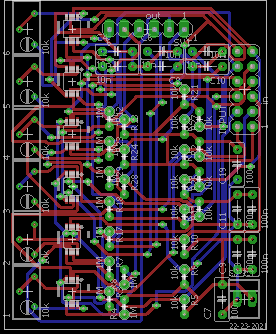
\includegraphics[scale=1.5]{textual-elements/hardware/TCC_INA}
\caption{PCB Project}
\end{figure}

\begin{figure}[!htpb]
\centering
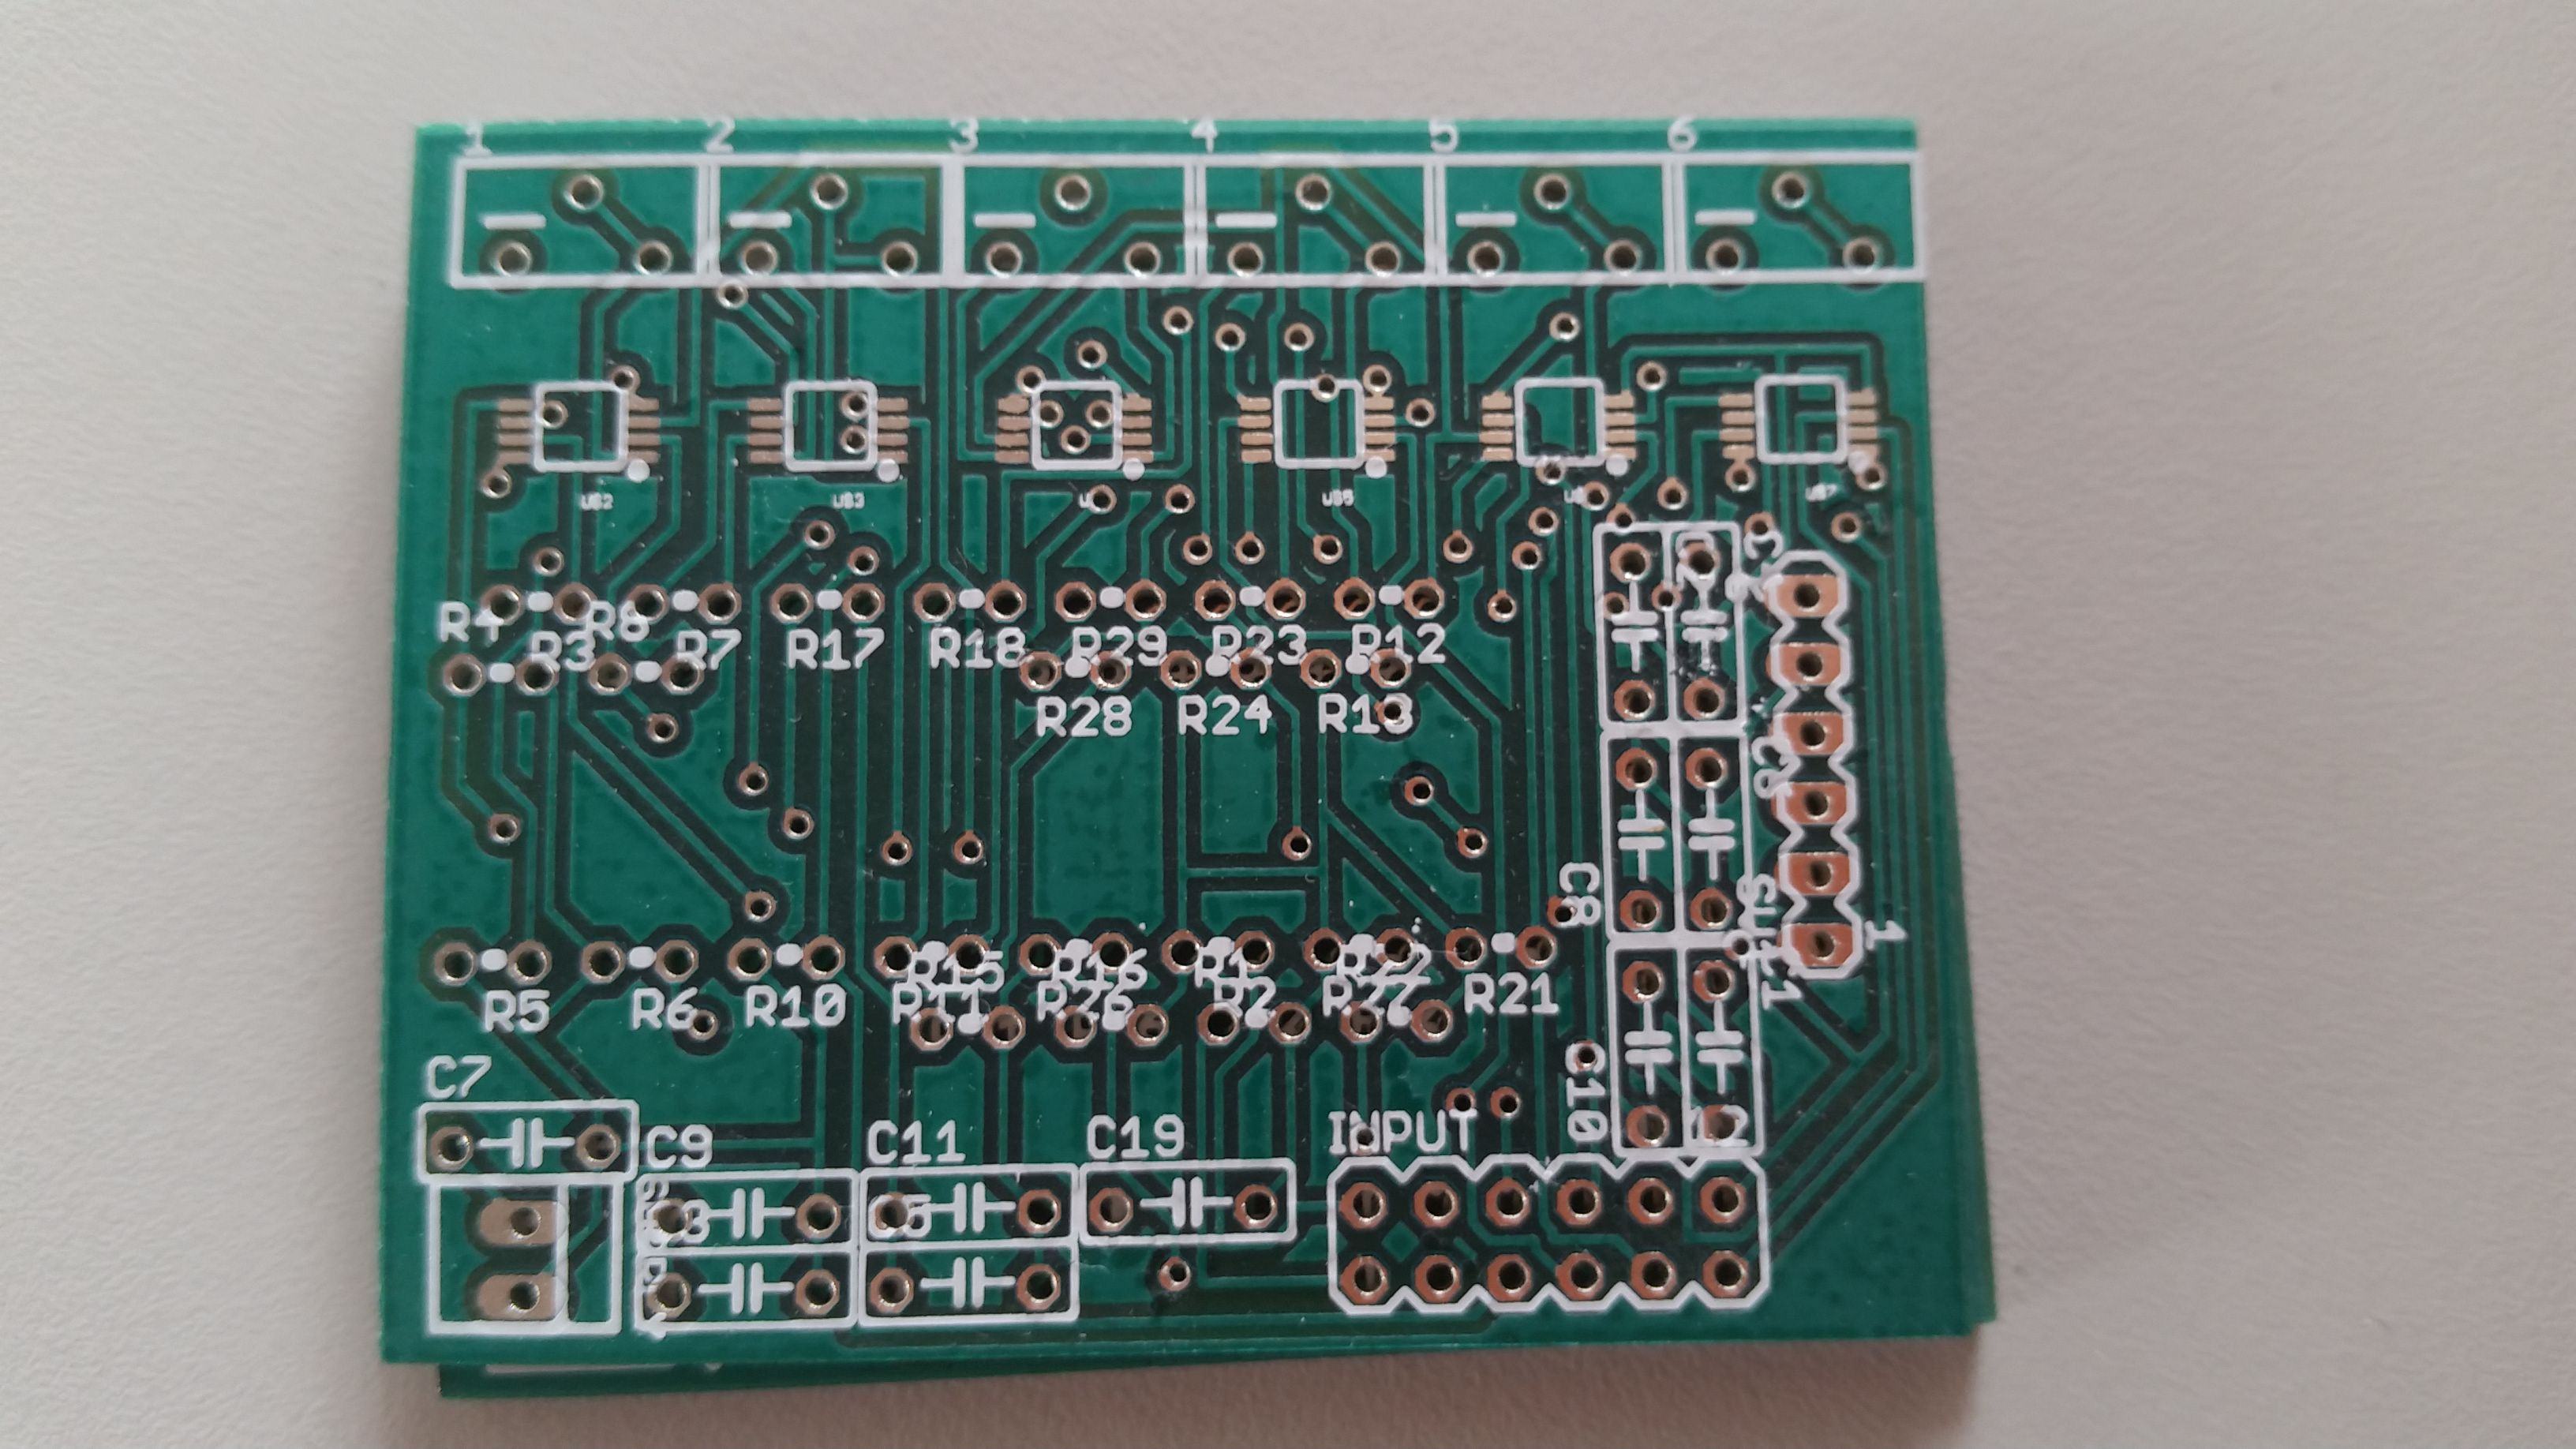
\includegraphics[scale=0.08]{textual-elements/hardware/INA_board}
\caption{PCB Project}
\end{figure}

On this project it was used:

\begin{itemize}
\item 6 Instrumental Amplifiers INA 326;
\item 6 10k$\Omega$ Trimmer Potentiometer;
\item 6 10nF Ceramic Capacitor;
\item 6 100nF x 50V Electrolitic Capacitor;
\item 12 10k$\Omega$ 5 Percent Tolerance Resistor;
\item 12 1M$\Omega$ 5 Percent Tolerance Resistor;
\item 1 6 positions Pin bar;
\item 1 12 positions dual track Pin bar;
\item 1 2 positions Pin bar;
\end{itemize}  

After soldering all the components it was performed some bench tests to verify the functionality of the amplifier circuit. The result showed us that the circuit attends the required function, amplifying the signal from a pick of 10mV to a pick of 1V, proving that the circuit is working perfectly and attending the demand of the project. After the bench test the system was connected to the pickup to verify if the guitar signal would be amplified as needed to the conversion process. The result was satisfactory and attended well the purpose to the project, as showed on image 6.  

\begin{figure}[!htpb]
\centering
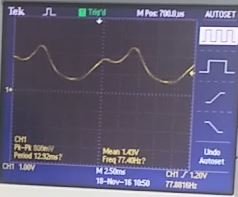
\includegraphics[scale=1]{textual-elements/hardware/INA_result}
\caption{INA Project Result}
\end{figure}

\subsection{TLV 4316}
The project of TLV 4316 started on the same way of the INA 326 project. It started verifying the datasheet 

\chapter{Firmware}

\section{Specifications}
\label{firmware-specifications}

The firmware is basically an analog sampler, all it has to do is sample six analog
channels, add a header (to identify the beginning and check continuity) and send it
through USB. The following sections present the requirements of the system, details
about the selection of the microcontroller and how the signal acquisition parameters
(set by registers) were obtained.

\subsection{Requirements}
\begin{itemlist}
  \item Super cheap
  \item 6 analog channels (more precision is better)
  \item High sample rate (at least 10 kHz for each channel, but ideally 44 kHz or more)
  \item Fast USB support, to send the data with headers
\end{itemlist}
Based on this requirements the minimum transfer speed can be calculated. Considering
that a header will be set for every 252 samples (42 for each channel) and
it has 4 bytes (3 of identification - to assure it is the header and not some
data - and a counter). Previewing the worst case, each sample is 2 bytes long.
The transfer rate given by \autoref{usb-generic-rate-equation}.

\begin{equation}
  \label{usb-generic-rate-equation}
  transfer\ rate = \left( \frac{channels * \frac{bytes}{sample} * \frac{samples}{package} + header\ size}{\frac{samples}{package}}  \right ) * f_{s} [B/s]
\end{equation}

Considering that $f_{s}$ has to be somewhere between 10 kHz and 50 kHz, the transfer
rate numerical result is given by \autoref{usb-numerical-rate-equation}.

\begin{equation}
  \label{usb-numerical-rate-equation}
  transfer\ rate = \left( \frac{6 * 2 * 252 + 4}{252}  \right ) * f_{s} = 12.0159 * f_{s} = 120.159\ to\ 600.794 [kB/s]
\end{equation}

USB transfer speed is usually referred in Mbps, which gives a range between
961.27 and 4806.34 Mbps. This is too high for serial communication (typical max of
1 Mbps) so we need to add a requirement for raw USB support, which allows \textit{bulk transfers}
that can a have transfer rate up to 12Mbps (USB full-speed standard).

It's still needed to choose or exact sample rate ($f_{s}$), but it is first necessary
select which hardware will be used.

\subsection{Microcontroller Selection}
There are too many microcontrollers that fit our requirements, but the most popular
and cheap one is clearly the ARM from ST called STM32F103C8T6 \cite{STM32F103},
and that is why it was selected. 

It has eight 12 bits ADC inputs (with 2 parallel channels), DMA for the ADCs and USB full-speed support. It's
also relatively fast (72 MHz clock, 32 bits architecture). All this for under 2 US\$
in a developing board from China (the actual $\mu$C is under 0.2 U\$). 

The board an it's pinout can be seen in \autoref{STM32F103-board}.

\begin{figure}[htb]
  \centering
  \caption{STM32F103C8T6 Board}
  \label{STM32F103-board}
  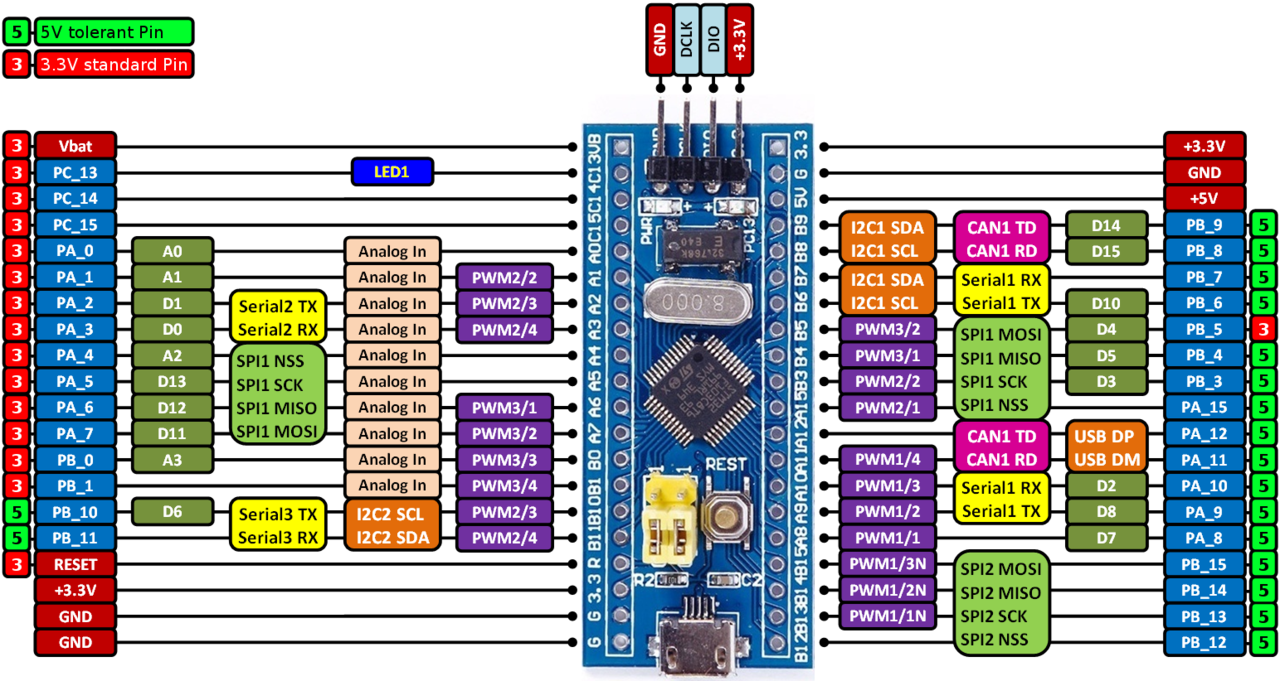
\includegraphics[scale=0.3]{images/STM32F103-board}
  \legend{Source: \citeonline{STM32F103-board-image}}
\end{figure}

\subsection{Sample Frequency}
\label{firmware-sample-frequency}
Usage of the ADCs for the selected $\mu$C can be optimized by using continuous sampling
mode in conjunction with DMA \cite[ch. 11]{STM32F103}. In this mode the sample frequency is controlled by a register
that sets the convolution time, which gives more precision the more ADC clock
cycles (longer) it takes to sample.

The first variable chosen for this setup is the ADC clock, which is set by dividing
the $\mu$C clock by 2, 4, 6 or 8. The ADC also has a maximum clock of 14 MHz. Taking in
account the  $\mu$C clock of 72 MHz, the highest possible value for the ADC clock is 12 MHz,
which is set by a divider value of 6. 

The last value to be chosen is the mentioned convolution time ($T_{c}$ is calculated as the selected
value plus 12.5 ADC clock cycles), which gives a sample frequency calculate by \autoref{ADC-sampling-time}.

\begin{equation}
  \label{ADC-sampling-time}
  f_{s} = \frac{ADC\ clock}{T_{c} + 12.5}  * \frac{ADCs}{channels} = \frac{12}{T_{c} + 12.5}  * \frac{2}{6}\ [MHz]
\end{equation}
\autoref{ADC-sampling-frequencies} shows the calculated results for each possible
register value (using \autoref{ADC-sampling-time}). Based on it the chosen sampling
frequency is 47.619 kHz. By using \autoref{usb-numerical-rate-equation} we can also
calculate the actual data transfer rate (for all channels, including header),
resulting in a total of 572,185 kHz. This last value will be used to test the USB communication.

\begin{table}[htb]
  \caption{ADC Sampling Frequencies}
  \label{ADC-sampling-frequencies}
  \begin{tabular}{c|c|c}
    \textbf{Register Value} & \textbf{Convolution Time [cycles]} & \textbf{Sampling Frequency [kHz]}\\
    \hline \hline
    000 & 1.5 & 285.71 \\
    \hline
    001 & 7.5 & 200 \\
    \hline
    010 & 13.5 & 153.85 \\
    \hline
    011 & 28.5 & 97.56 \\
    \hline
    100 & 41.5 & 74.07 \\
    \hline
    101 & 55.5 & 58.82 \\
    \hline
    \textbf{110} & \textbf{71.5} & \textbf{47.62} \\
    \hline
    111 & 239.5 & 15.87 \\
  \end{tabular}
  \legend{Source: authors}
\end{table}

\section{Implementation}
\label{firmware-implementation}

\subsection{First Attempt}
We first tried to build our firmware from scratch, using the tools given by the
manufacturer, essentially a set of driver abstractions (HAL drivers). The problem
found is that these abstractions are too slow, and don't work when the firmware
uses the hardware close to it's limits (as we do for both transfer and sampling rates).

\subsection{Second Attempt}
In our research we found a high quality open source project called MiniScope \cite{MiniScope},
in which a few options of low budget DIY digital scope (using different $\mu$Cs) are
presented. One of the $\mu$Cs used by MiniScope is the one we selected, so for our
implementation we took it's firmware as a base project. In this project the author
claims to sample and transfer two channels at 461 kHz (but 8 bits only), which is
very close to our needs (we need a little more transfer but much less sampling speed).

\subsection{IDE}
As we take MiniScope as a base project we will be using the same IDE as it, named
CooCox \cite{CooCox}. It has a full set of tools, and it's completely free (no limitations).

\subsection{Modifications}
The base project samples 2 channels at a different speed, bit rate and does not
add any headers to the data. It also has some code to answer a few commands. It
was as simple as setting up the registers for 6 channels, changing the sample size,
placing our already chosen speed (\autoref{firmware-sample-frequency}) and removing
any unused code. \\
The act of changing the sample size was not done by registers. MiniScope was already
sampling with 12 bits, but it was ignoring the least significant ones when filling
the USB buffer. What we have done is to change the bits alignment and putting all
the data received from the ADC to the USB buffer.

\subsection{Testing}
At first an attempt using the OS (Windows at that time, later Ubuntu) default driver
as made. That did not work well, as it is too generic and thus slow. \\
At a second try, a simple libusb \cite{libusb} program was built to test the transfer
rate (calculated in \autoref{firmware-sample-frequency}). The reported result is
almost perfectly the calculated one.

\subsubsection{Repository}
Again, all code is available at GitHub \cite{guitar-digitizer-firmware}.



\part{Software}

% TODO: include chapters, ex.:
\chapter{Tools Selection}
\label{tools-selection}

\section{Top Level Requirements}
The exact implementation of each of the items will be discussed later, but to
simply set our requirements a general list of them is:

\begin{itemlist}
  \item Desktop GUI
  \item Efficient signal processing (for pitch detection)
  \item Real time graph visualization of the signals (oscilloscope like)
  \item Access to \textit{libusb} \cite{libusb} API
  \item Access to MIDI API
\end{itemlist}

\section{Language Choice}

\subsection{Java}
The first choice was Java, as it meets all requirements. Desktop GUI can be done
using Swing, a good library for pitch detection is also available (called TasosDSP \cite{TarsosDSP}).
There is also a binding to libusb called usb4java and native MIDI support. \\
Following that idea a functional prototype was built, but a few problems came to rise.
The first is that usb4java high-level API had bugs and was not working correctly.
The solution was to fall back to the lower level API, but that made things much
more complicated as threading and synchronization problems had to be dealt with.
There was no good library for
real time visualization either, which made really hard to both debug and tune the
frequency detection algorithm. On top of that Swing is at least non-pleasant
compared to more modern UI programming, so a second approach came to be.

\subsection{JavaScript}
In alignment with both current work experience and world programming tendencies
JavaScript was taken as a choice. We will see that requirements fit much better now,
for the following reasons. \\
For the desktop GUI, JavaScript has a few nice and mature Desktop GUI frameworks,
like Electron and NW.js. \\
JavaScript is an interpreted language, and for that has a low efficiency when
compared to C++ or Java. That is huge problem, but there is an easy overcome. As
this project tries to build a desktop application, Node.js will be used ultimately,
and it has support for C++ bindings. That means the JavaScript code can call a
compiled C++ library to calculate the pitch, thus solving the problem. \\
Graph visualization should not be a problem either as there are a lot of libraries
for that. \\
The most problematic requirement in Java was \textit{libusb} support. It is available
in JavaScript using \textit{node-usb} \cite{node-usb}, and a few simple tests
returned good results with a much simpler API. MIDI was also tested and worked just fine.

\section{Desktop Framework}
Now that JavaScript is set as our final selection we need an environment to run
it. There are two already listed really mature and popular choices: Electron and NW.js. \\
At first Electron was used to build a test application, because it is the most popular
of the two (in fact even the editor used to write this words is built with it),
but the pitch detection call was running slowly. As a mater of fact it was running
much faster using pure JS code rather than the C++ library. A deeper research
was needed, and the way Electron worked was getting in our way, but first it's
necessary to know what Node.js is.

\subsection{Interpreter}
JavaScript is a interpreted language and thus needs an interpreter. The most
common one is Google V8, which happens to be the same one used in most web
browsers as well as in Node. The difference between browsers and Node is simply
the API that comes with them. Web needs firstly to access the UI (html) and ways to
modify it, it also needs secure and limited access to hardware and internet calls.
Of course that means web JavaScript code cannot use C++ libraries directly. \\
On the other hand Node is a more pure version of V8, it also gives the possibility
to write and call C++ code (feature needed for this project), which ultimately
makes it as capable as any desktop
program can be. Node also comes with a hand-full set of native resources (like
file system and full communication access), but it does \textbf{not} provide
any kind of GUI. Knowing that it is possible to have a better understanding on
how the two desktop environments work.

\subsection{Electron}
Electron by design has at least two processes running \cite{ElectronVsNW},
one for the "web" and other
for Node access. The answer for how the web process access native resources is
also to why the execution of the C++ processing library was slow: it uses
inter-process communication (IPC). IPC makes things a lot slower, which ultimately
makes impossible to use Electron in this project.

\subsection{Node Webkit}
Differently from Electron, NW.js \cite{NWjs, ElectronVsNW} takes the Node environment
and combines it with Chromium into a single process, removing the use of IPC.
Initial tests reported that the pitch detection library has fast
execution as expected.

\section{Architectural Tools}
NW.js will go only as far as to give access to both Node and DOM API's. But that
is too crude, and not what we wanted by given up on Java Swing. Again based on
current work experience and world tendencies the setup chosen is React + Redux. \\
React \cite{React} is a library created by Facebook and world wide used for UI applications.
It uses a declarative component-based system that makes it easy to build scalable
and reusable code.\\
React only go as far to help building the UI, but we also need to pass the state
of the application to the UI components, and that is where Redux \cite{Redux} comes in.
It keeps all the application state stored in a single place, described by transition
functions. That makes the storage system easy to be tested and used, because all
actions (that modify the state) must be well defined and it doesn't rely on the
UI (React), making it easy to test.\\
\autoref{react-redux-diagram} shows the flow of an application that uses
React + Redux. It is obvious to see the simplicity it has, a single path must be followed.
This simplicity is what makes it much easier to use against other frameworks like
Java Swing. \\
There is still the choice of the visual library to use, and the chosen one is
Semantic UI React \cite{semantic-ui}. It has some nice and robust React components
to build a well designed application.

\begin{figure}[htb]
  \centering
  \caption{React Redux Flow Diagram}
  \label{react-redux-diagram}
  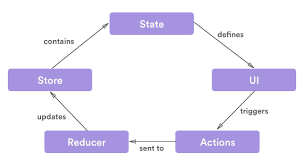
\includegraphics[scale=0.5]{images/react-redux-diagram.png}
  \legend{Source: \citeonline{react-redux-diagram-source}}
\end{figure}

\section{Fast Signal Processing}
Pitch detection is a heavy problem to solve, and good implementations are time
consuming, so we need efficiency to run it real-time. The library already said
to be used didn't actually existed, the only one available was a pure JavaScript
library \cite{pitchfinder} which is not suitable for this project. The solution
was to build our own library based on both the pure JavaScript one and TarsosDSP
\cite{TarsosDSP}. Implementation details discussed further on \autoref{pitch-detection}.

\section{Real Time Visualization}
There are lots of charting libraries available for use with web interfaces (and
by extension NW.js), unfortunately none was good fit for real time high density
signals such as audio. The solution was again to build one, since all other things
are looking to run smoothly in JavaScript, implementation details on \autoref{data-visualization}.

\chapter{Pitch Detection}
\label{pitch-detection}

Pitch detection is simply frequency detection with the restriction of note quantization,
\autoref{notes-frequencies} shows the base frequency for each of the 12 existent
notes. Multiples of the same frequency are seen as the same note on a different
range, known as octave.

\begin{table}[htb]
  \begin{center}
    \ABNTEXreducedfont
    \caption[Notes Frequencies]{Notes Frequencies}
    \label{notes-frequencies}
    \begin{tabular}{c|c}
      \hline
      Note Name & Frequency\\
      \hline
      A & 440.00 \\
      A\# & 466.16 \\
      B & 493.88 \\
      C & 523.25 \\
      C\# & 554.37 \\
      D & 587.33 \\
      D\# & 622.25 \\
      E & 659.25 \\
      F & 698.46 \\
      F\# & 739.99 \\
      G & 783.99 \\
      G\# & 830.61 \\
      \hline
    \end{tabular}
    \legend{Source: made by authors}
  \end{center}
\end{table}

Even though the quantization makes things simpler it's still a hard task, even
more for instruments whereas there is the presence of harmonic series. Harmonic
series notes are multiples of the fundamental frequency (most important
note) produced by integer sections of the instrument vibration. \autoref{harmonic-series}
shows an visual representation of why there exist. The existence of them as well
as the presence of both inter-signal and white noise makes necessary the use of
non-trivial algorithms for pitch detection, and two of them will be discussed next.


\begin{figure}[htb]
	\caption{Harmonic Series}
  \label{harmonic-series}
	\begin{center}
    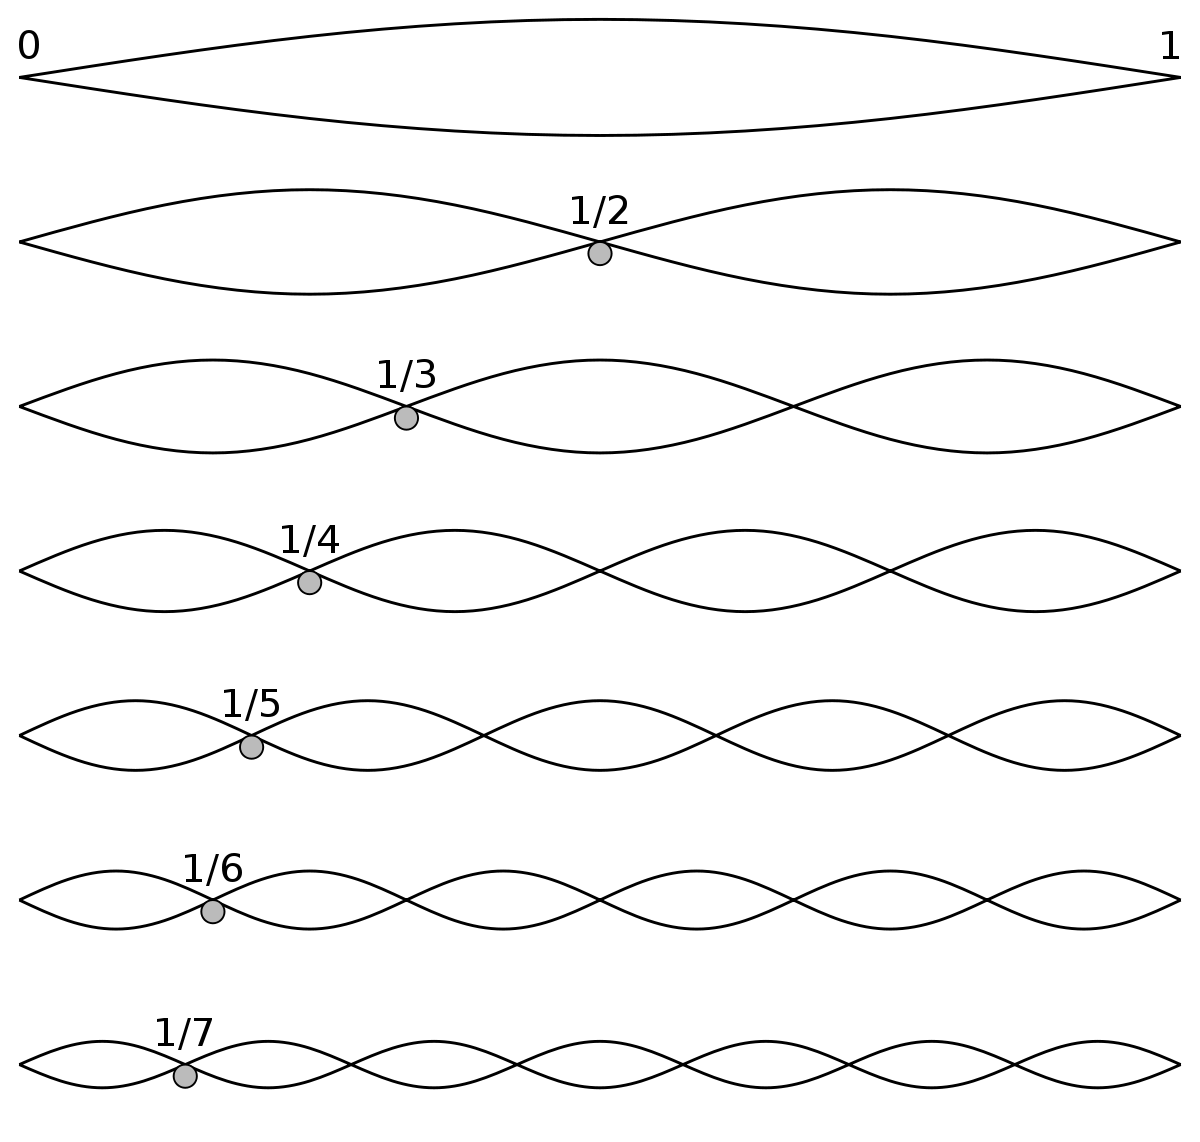
\includegraphics[scale=0.15]{images/harmonic-series.png}
	\end{center}
  \legend{Source: \citeonline{harmonic-series-figure-source}}
\end{figure}

\section{YIN algorithm}

Autocorrelation is a well know function to calculate a signal's fundamental
frequency, but it gives too much error for this project use case. YIN \cite{YINArticle}
is a method that uses a few improvements to the autocorrelation method, achieving
a much higher precision. The algorithm can be divided in 6 steps, as follows:

\begin{enumerate}
  \item Autocorrelation function
  \item Difference function
  \item Cumulative mean normalized difference function
  \item Absolute threshold
  \item Parabolic interpolation
  \item Best local estimate
\end{enumerate}

\chapter{Data Visualization}
\label{data-visualization}

The objective of data visualization is to live debug and tune both hardware gain
and algorithms control constants. The ideal case is to have both real time chart
as well as a buffered/triggered one, essentially something like an oscilloscope.
That has to be performant for real time audio signals, sampled at more than 47 kHz.\\
There are a great amount of JavaScript DOM libraries for charting, but most of
them are too automatic or have too much details, making them too slow for our need.
The solution was to build our own library for that, again available as an open source
project at both GitHub and npm \cite{react-plotter}.

\section{Requirements}
\label{data-visualization-requirements}
\begin{itemlist}
  \item Be a React Component
  \item Automatic calculations for array input
  \item Option for triggering
  \item Option for buffering
  \item Minimum Redraw
  \item Fixed Height/Width
\end{itemlist}

\section{Algorithm}
Triggering and buffering are achived by using a filter that only calls the ploting
function when the options are met. This filter is simply the function called to
add data, and it is represented by \autoref{react-plotter-add-diagram}. \\
\begin{figure}[htb]
  \caption{Add Function Diagram}
  \label{react-plotter-add-diagram}
  \centering
  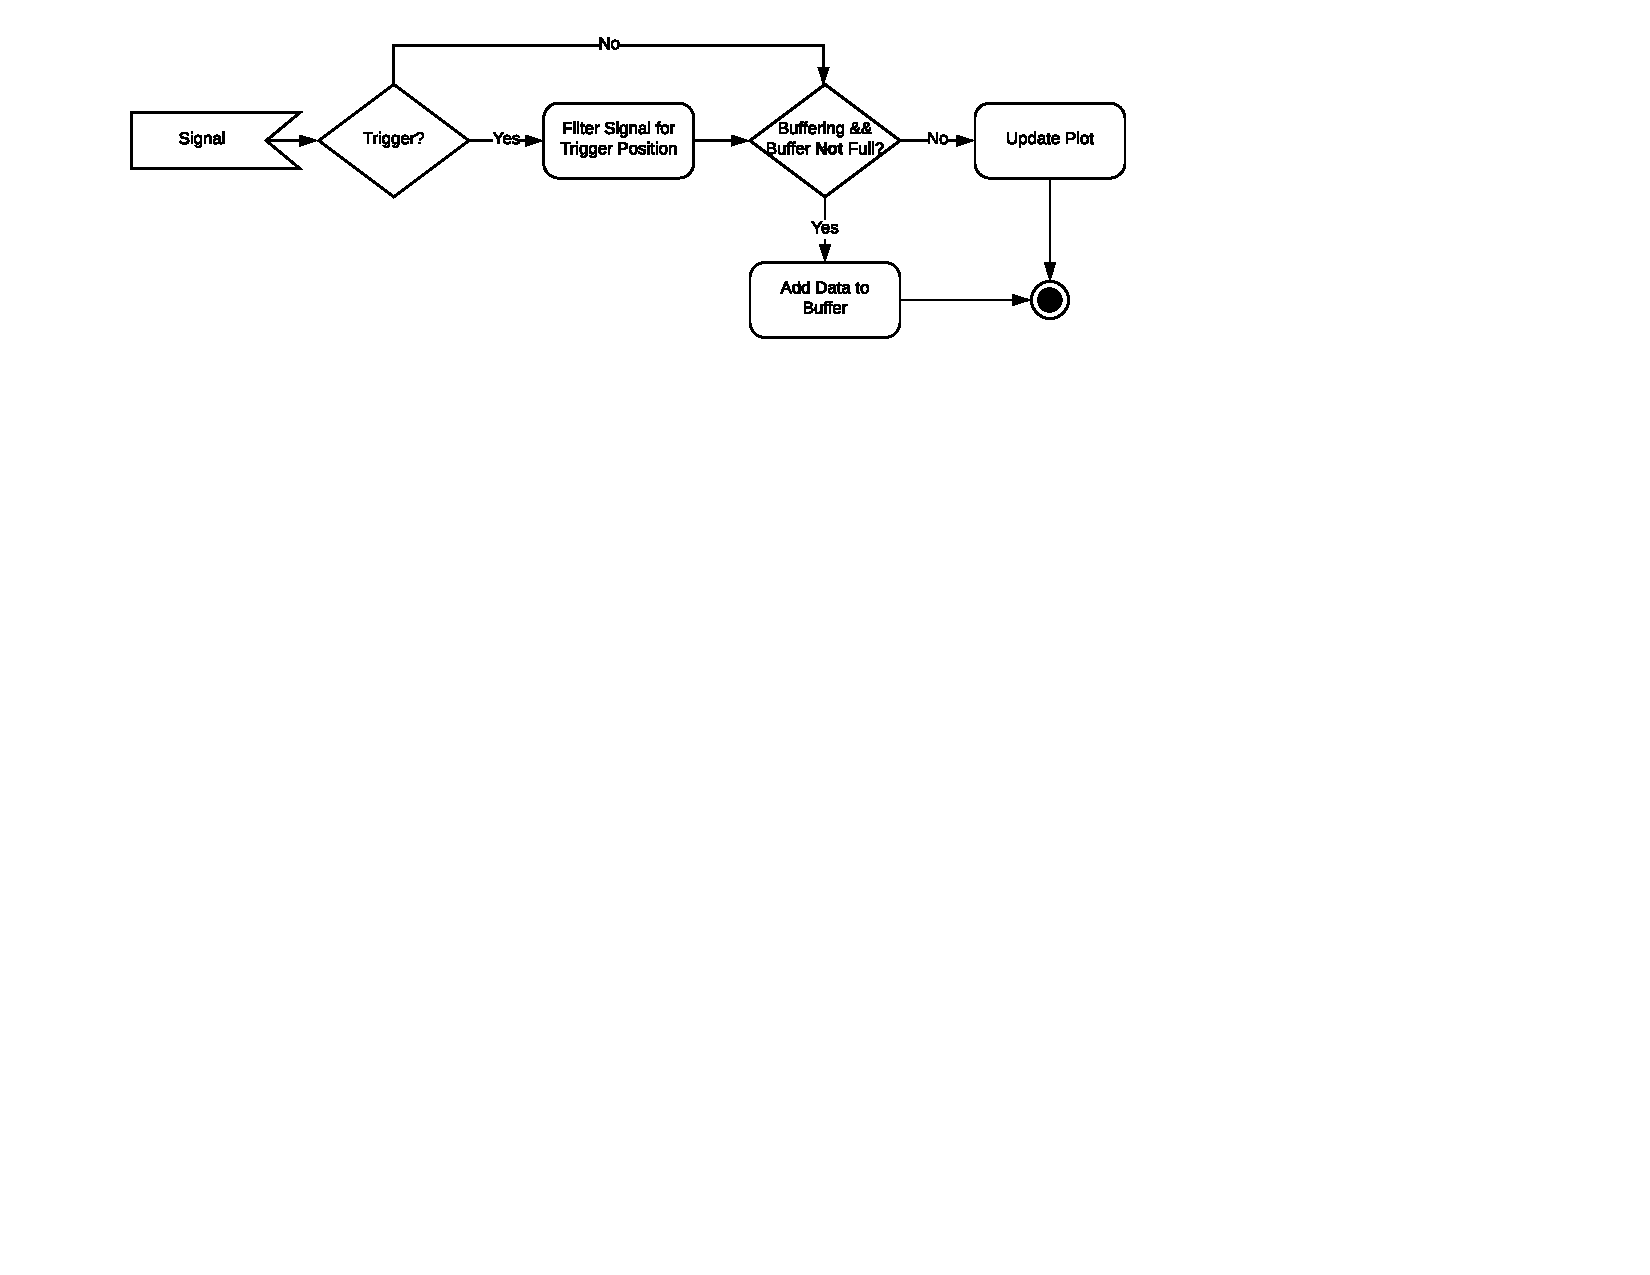
\includegraphics[scale=0.35]{images/react-plotter-add-diagram.pdf}
  \legend{Source: made by authors}
\end{figure}
For the actual drawing a triple buffer technique is used, one for holding the last
state (called plotBuffer), on for drawing (called drawingBuffer) and finally the
one actually rendered (called canvas). That last one is needed so the arrows don't
get saved on the drawing scene. \\
For linear plot time a translation is established, in a way that only the new
points will be drawn, the past ones are only translated to the left. The steps
of the algorithm are as follow:
\begin{enumerate}
  \item Clear drawingBuffer
  \item Copy plotBuffer to drawingBuffer translating (removing) extra data
  \item Draw new data on drawingBuffer
  \item Copy drawingBuffer to plotBuffer
  \item Copy plotBuffer to canvas
  \item Draw arrows on canvas
\end{enumerate}

\section{Implementation}
Using the listed requirements (\autoref{data-visualization-requirements}) a minimum
API is built as a React component. Being such all it gives is a set of properties,
for which the chart is drawn (when needed), they are listed in \autoref{react-plotter-props}.
\begin{table}[htb]
  \ABNTEXreducedfont
  \caption[React Plotter Props]{React Plotter Props}
  \label{react-plotter-props}
  \centering
  \begin{tabular}{c|c|c}
    \textbf{Property} & \textbf{Type} & \textbf{Description} \\
    \hline
    style &	Function & Style function (called to print the data) \\
    \hline
    {[trigger]} &	number & Use trigger \\
    \hline
    {[onlyFull=true]}	& bool & When using trigger it tells if the view should \\
                      &      & wait for a complete dataset before updating \\
    \hline
    {[width=300]} &	number \\
    \hline
    {[height=150]} & number \\
    \hline
    {[initialData=[ ]]} & number{[ ]} \\
    \hline
    {[appendData=[ ]]} & number{[ ]} \\
    \hline
    {[dataSize=100]} & number \\
    \hline
    {[pixelSkip=1]} &	number &	Pixels between points \\
    \hline
    {[max=100]} &	number & Maximum Y Value \\
    \hline
    {[min=-100]} & number & Minimum Y Value \\
    \hline
    {[useMean=true]} & bool & Use mean calculation, otherwise median  \\
  \end{tabular}
  \legend{Fonte: \citeonline{react-plotter}}
\end{table}
The style property is a function that is called to render each point. Two styles
were built, a line plot (points are connected by a straight line) and a digital
plot (digital signal standard chart, not used in the final version of this project).

\section{Results}
The results are more than satisfactory, tested to be able to run multiple plots
of audio speed signals at the same time without much effort. \autoref{plot-real-time}
and \autoref{plot-triggered} show how the visualization looks on the
project, but full details and working examples are also available at GitHub
\cite{react-plotter}.

\begin{figure}[htb]
 \centering
  \begin{minipage}{0.4\textwidth}
    \centering
    \caption{Real Time Plot} \label{plot-real-time}
    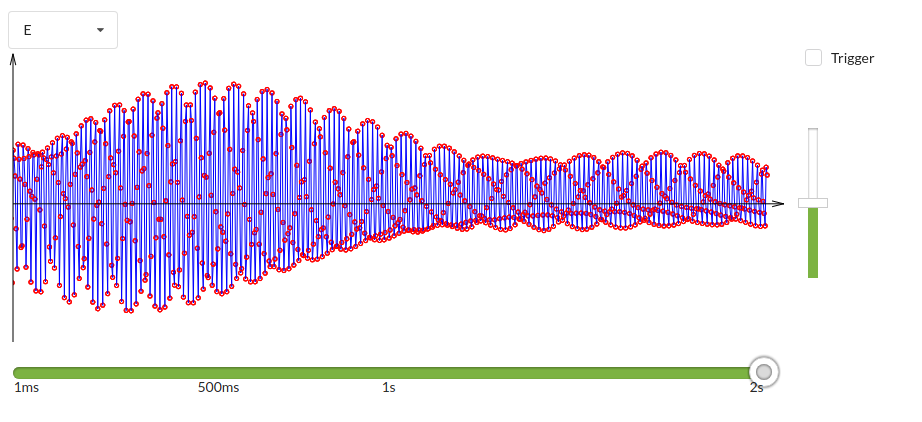
\includegraphics[scale=0.22]{images/snapshots/plot-real-time.png}
    \legend{Source: authors}
  \end{minipage}
  \hfill
  \begin{minipage}{0.4\textwidth}
    \centering
    \caption{Triggered Plot} \label{plot-triggered}
    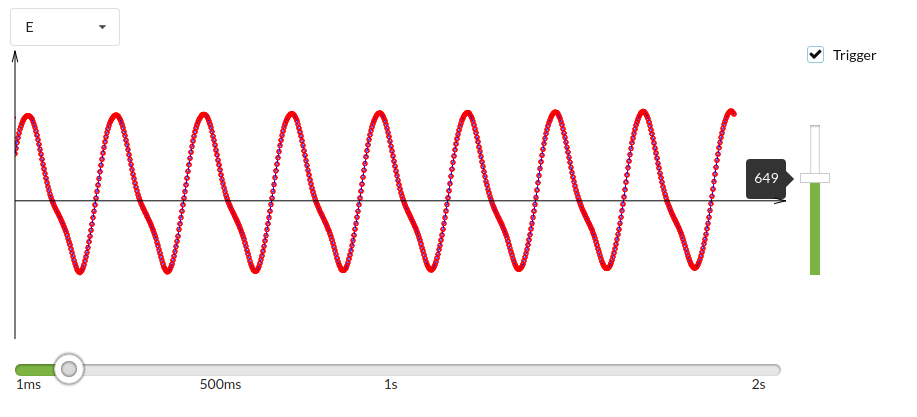
\includegraphics[scale=0.22]{images/snapshots/plot-trigger-E.png}
    \legend{Source: authors}
  \end{minipage}
\end{figure}



\chapter{Experiments and Discussions}
For the assessment of the system we performed the measurements listed below
\footnote{
  Unfortunately one of our input channels is not functioning (corresponding to the
  D string), due to a hardware problems (not identified at the timing of writing this document),
  hence it will be ignored. B string signal has DC noise,
  due to resistor imprecisions (not fixed at the time of these experiments),
  which limits the signal peak to peak value, and so it will have poor performance.
}.
Results and discussions are presented in the following sections.

\begin{itemize}
  \item Single Note Accuracy
  \item Chord Accurracy (E and Am)
  \item Chromatic Scale Error
  \item Pluck Counting
\end{itemize}


\section{Single Note Accuracy}
This test is done by hitting a single note in a single string and checking if the correct
frequency is detected. Notes were chosen in order to consider a broad frequency band,
as presented in \autoref{single-note-expected-result}. The amount of detected notes is
not considered in this experiment. \autoref{single-note-result} and \autoref{single-note-accuracy}
present the results. MacLeod presents lower errors.

\begin{table}[htb]
  \begin{center}
    \ABNTEXreducedfont
    \caption[Single Note Expected Result]{Single Note Expected Result}
    \label{single-note-expected-result}
    \begin{tabular}{c | c | c}
      \hline
      String & Frequency(Hz) & Note (name and number)\\
      \hline \hline
      E (6) & 493.9 & B4 (71) \\ \hline
      A (5) & 370 & Gb4 (66) \\ \hline
      G (3) & 293.7 & D4 (62) \\ \hline
      B (2) & 164.8 & E3 (52) \\ \hline
      e (1) & 123.5 & B2 (47) \\ \hline
    \end{tabular}
    \legend{Source: authors}
  \end{center}
\end{table}

\begin{table}[htb]
  \begin{center}
    \ABNTEXreducedfont
    \caption[Single Note Result]{Single Note Result}
    \label{single-note-result}
    \begin{tabular}{c | c | c | c | c}
      \hline
      String & MacLeod Mean (Hz) & MacLeod Standard Deviation & YIN Mean (Hz) & YIN Standard Deviation\\
      \hline \hline
      E (6) & 495.27 & 0.04 & 489.81 & 0.012 \\ \hline
      A (5) & 379.00 & 0.13 & 368.09 & 1.27 \\ \hline
      G (3) & 298.28 & 1.59 & 301.43 & 0.60 \\ \hline
      B (2) & 167.00 & 0.04 & 164.01 & 0.08 \\ \hline
      e (1) & 124.47 & 0.16 & 121.13 & 0 \\ \hline
    \end{tabular}
    \legend{Source: authors}
  \end{center}
\end{table}


\begin{figure}[!htpb]
  \centering
  \caption{Strings Single Note Accuracy}
  \label{single-note-accuracy}
  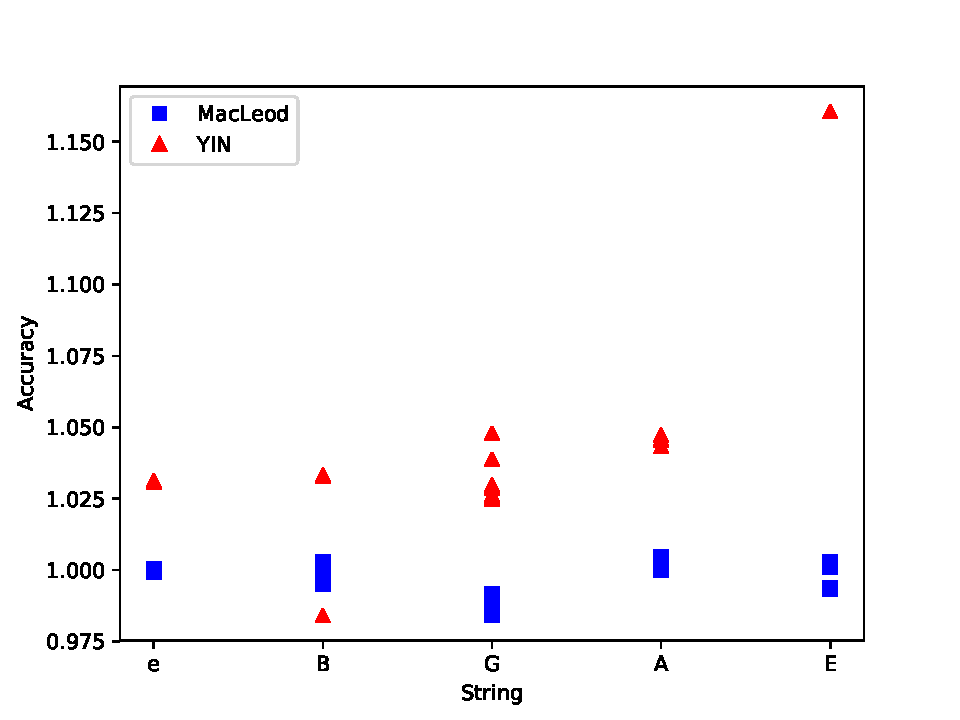
\includegraphics[scale=0.85]{images/measurements/single-note-acc-2}
  \legend{Source: Authors}
\end{figure}

\section{Chord Accuracy (E and Am)}
This experiment aims to assess the performance of the system when simultaneous notes at multiple string are played.
The adopted chords are the E major (E) and A minor (Am). The E chord has it's lower note on
the twelfth fret, to cut off very low frequencies. The Am chord has it's lower note
on the fifth fret, and so lower frequencies.
The error rate and standard deviation were calculated for both cases. The error rate is given by
\autoref{chord-accuracy-equation}. The result can be seen at \autoref{e-chord-error} and \autoref{am-chord-error}, where the
error is given in percentage and the standard deviation in absolute values.
YIN presents lower error, except at low frequencies where it present large error rates.

\begin{equation}
  \label{chord-accuracy-equation}
  Accuracy = \frac{Mean - Expected\ Value}{Expected\ Value} = \frac{\sum x}{Length * Expected\ Value} -1
\end{equation}

\begin{figure}[!htpb]
  \centering
  \caption{Am chord error}
  \label{am-chord-error}
  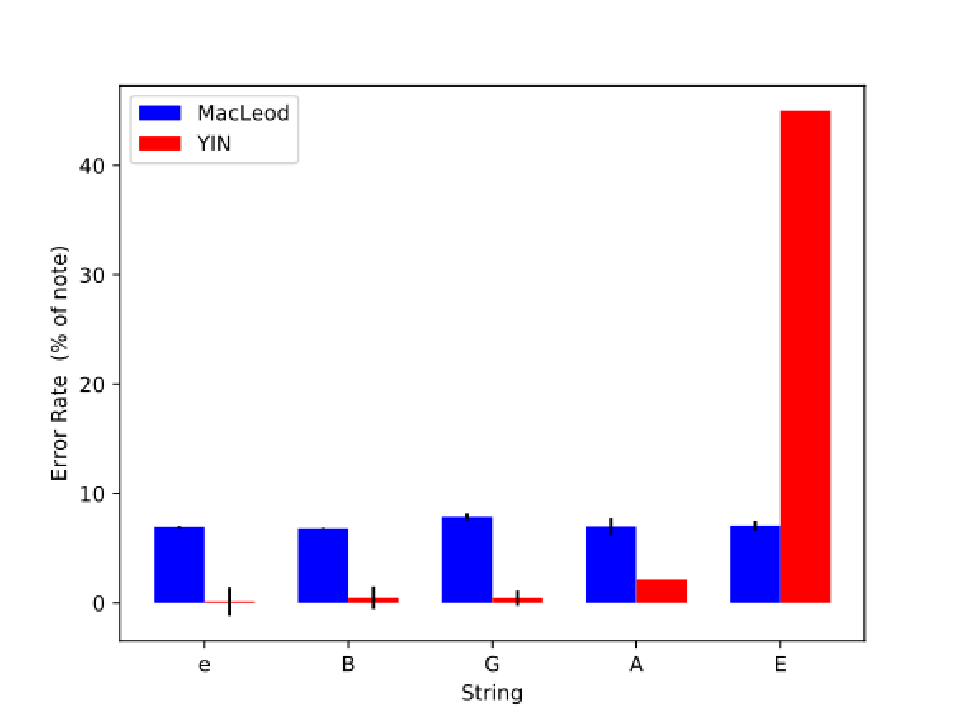
\includegraphics[scale=0.85]{images/measurements/am-chord-error}
  \legend{Source: Authors}
\end{figure}

\begin{figure}[!htpb]
  \centering
  \caption{E chord error}
  \label{e-chord-error}
  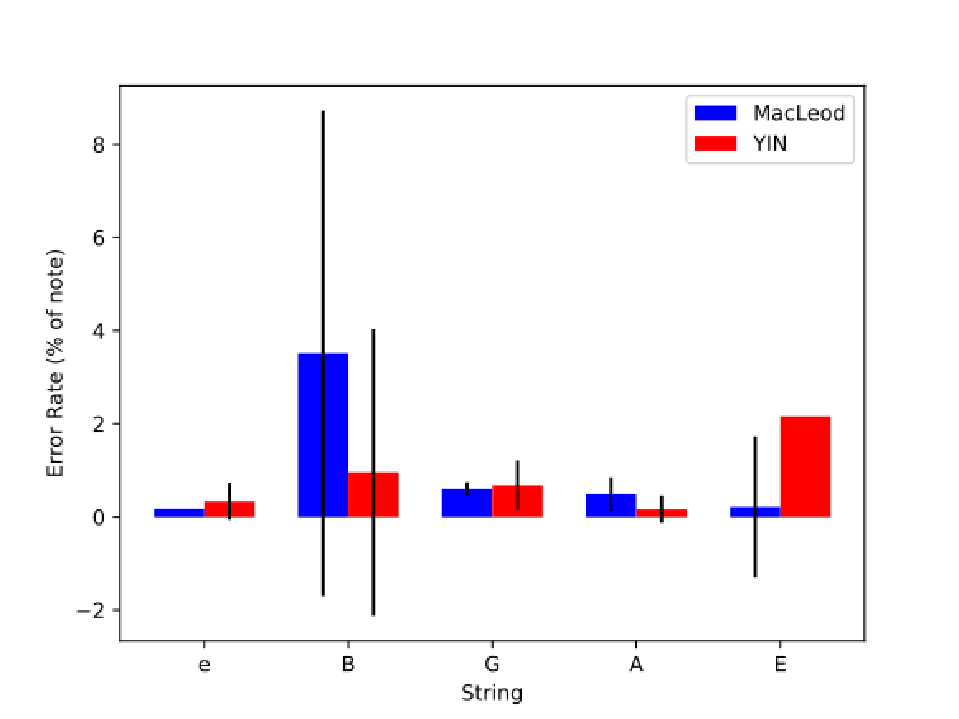
\includegraphics[scale=0.85]{images/measurements/e-chord-error}
  \legend{Source: Authors}
\end{figure}

\section{Chromatic Scale Error}
This experiment aims to assess the performance of the system on detection of notes over time.
Each string is played separately by plucking 5 consecutive
notes (e.g. A, A\#, B, C and C\#) at the speed of approximately 4 notes/s, which can be
considered an usual speed for guitar playing. To avoid pluck miss-detections in this test, repeated
notes are grouped into a single detection. The measurements were then compared with the
expected output, and any miss-detection counted. This test was repeated five times,
and the mean was taken as the error rate, calculated by dividing the number of 
errors by the total number of distinct detected notes. Results in \autoref{chromatic-scale-error}
show that MacLeod presents lower errors in this experiment.

\begin{figure}[!htpb]
  \centering
  \caption{Chromatic scale error}
  \label{chromatic-scale-error}
  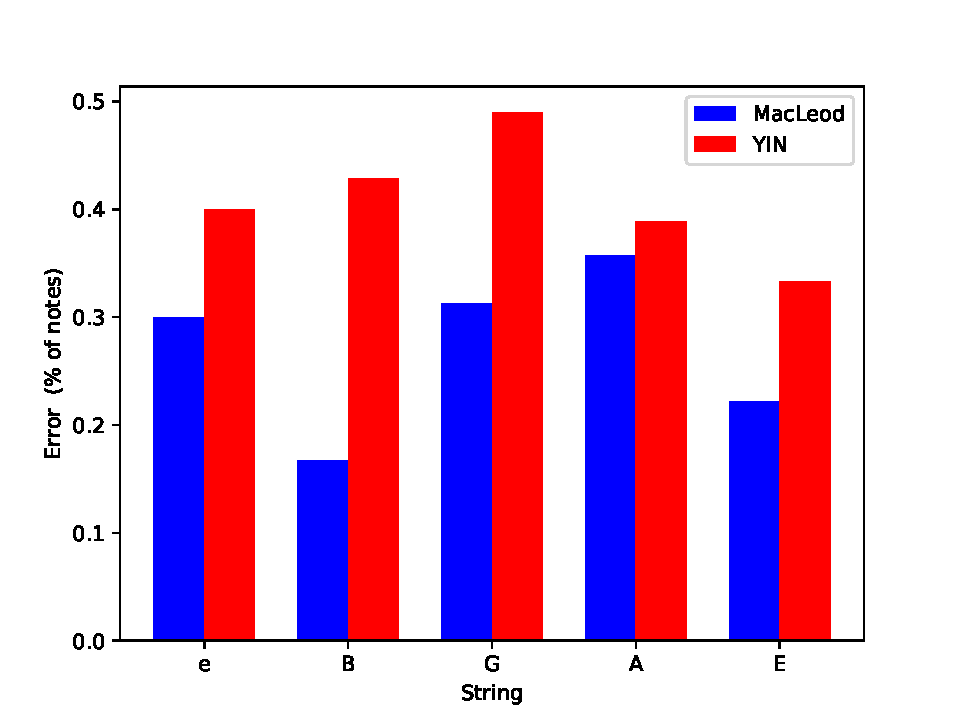
\includegraphics[scale=0.85]{images/measurements/chromatic-scale-error}
  \legend{Source: Authors}
\end{figure}

\section{Pluck Counting} \label{pluck-counting}
In this experiment, several trials of the following procedure are performed for different notes
from the first up to the tenth fret, for all strings: a single note is played 20 times in a row
at a 4 notes/s timing. Thus, the expected global mean of the pluck counting, considering, each
different played note is 20. The obtained values for the MacLeod and YIN were, respectively,
29.9 and 27, corresponding to a 42\% average error. This large error suggests that the simple
amplitude detection by taking the AC mean of the current sampled window is not enough to correctly
detect amplitude changes and more effective methods can be explored, such as \textit{onset detection}.

\section{Discussions}
Strings Single Note Accuracy test provided satisfactory results (\autoref{single-note-accuracy}).
This limited the channel gain which ultimately made this
channel results lower than the others. The same analysis is true for
all other experiments.

Both the chord detection experiments (\autoref{am-chord-error}, \autoref{e-chord-error}) gave reasonable results, but they
show that our system still has lots of room for improvement. The exception is for
the E string error on the Am chord using the YIN algorithm. The reason
for this is that YIN is not working well for low frequency notes, because
it still needs a greater period (samples) for analysis, which is not currently
possible due to processing time limitations - but a solution is proposed at
the next chapter.

The chromatic scale results (\autoref{chromatic-scale-error}) show that our system is not working well along time.
By using a small period of measurement (so it can run at real-time) the range
where a note is changing to the next one is misread as an incorrect result.
This is a big problem for music annotation, but has the same solution as above,
which needs performance improvement.

The last test (\autoref{pluck-counting}) also shows our time related issues,
that, although being natural, still need to be dealt with, for the same reason above, transitions
through time that need a larger sample period to work well, also a better algorithm to detect
amplitude changes. The plucking errors are due to the amplitude detection.


% ----------------------------------------------------------
% Conclusion (no numeration, but present in summary)
% ----------------------------------------------------------
\chapter*[Conclusion]{Conclusion}
\addcontentsline{toc}{chapter}{Conclusion}
% ----------------------------------------------------------

\lipsum[31-33]


% ------------------------------------------------------------------------
\postextual % POST TEXTUAL ELEMENTS
% ------------------------------------------------------------------------

\bibliography{post-textual-elements/references}

%\glossary

% \begin{appendicesenv}

% Print page with appendices title
\partappendices

\chapter{Quisque libero justo}

\lipsum[50]

\chapter{Nullam elementum urna vel imperdiet sodales elit ipsum pharetra ligula
ac pretium ante justo a nulla curabitur tristique arcu eu metus}
\lipsum[55-57]

\end{appendicesenv}


\begin{annexesenv}

% Imprime uma página indicando o início dos anexos
\partannexes

\chapter{INA 326 complete Schematic.}

\begin{figure}[!htpb]
  \centering
  \caption{INA 326 Complete Schematic}
  \label{INA-complete-schematic}
  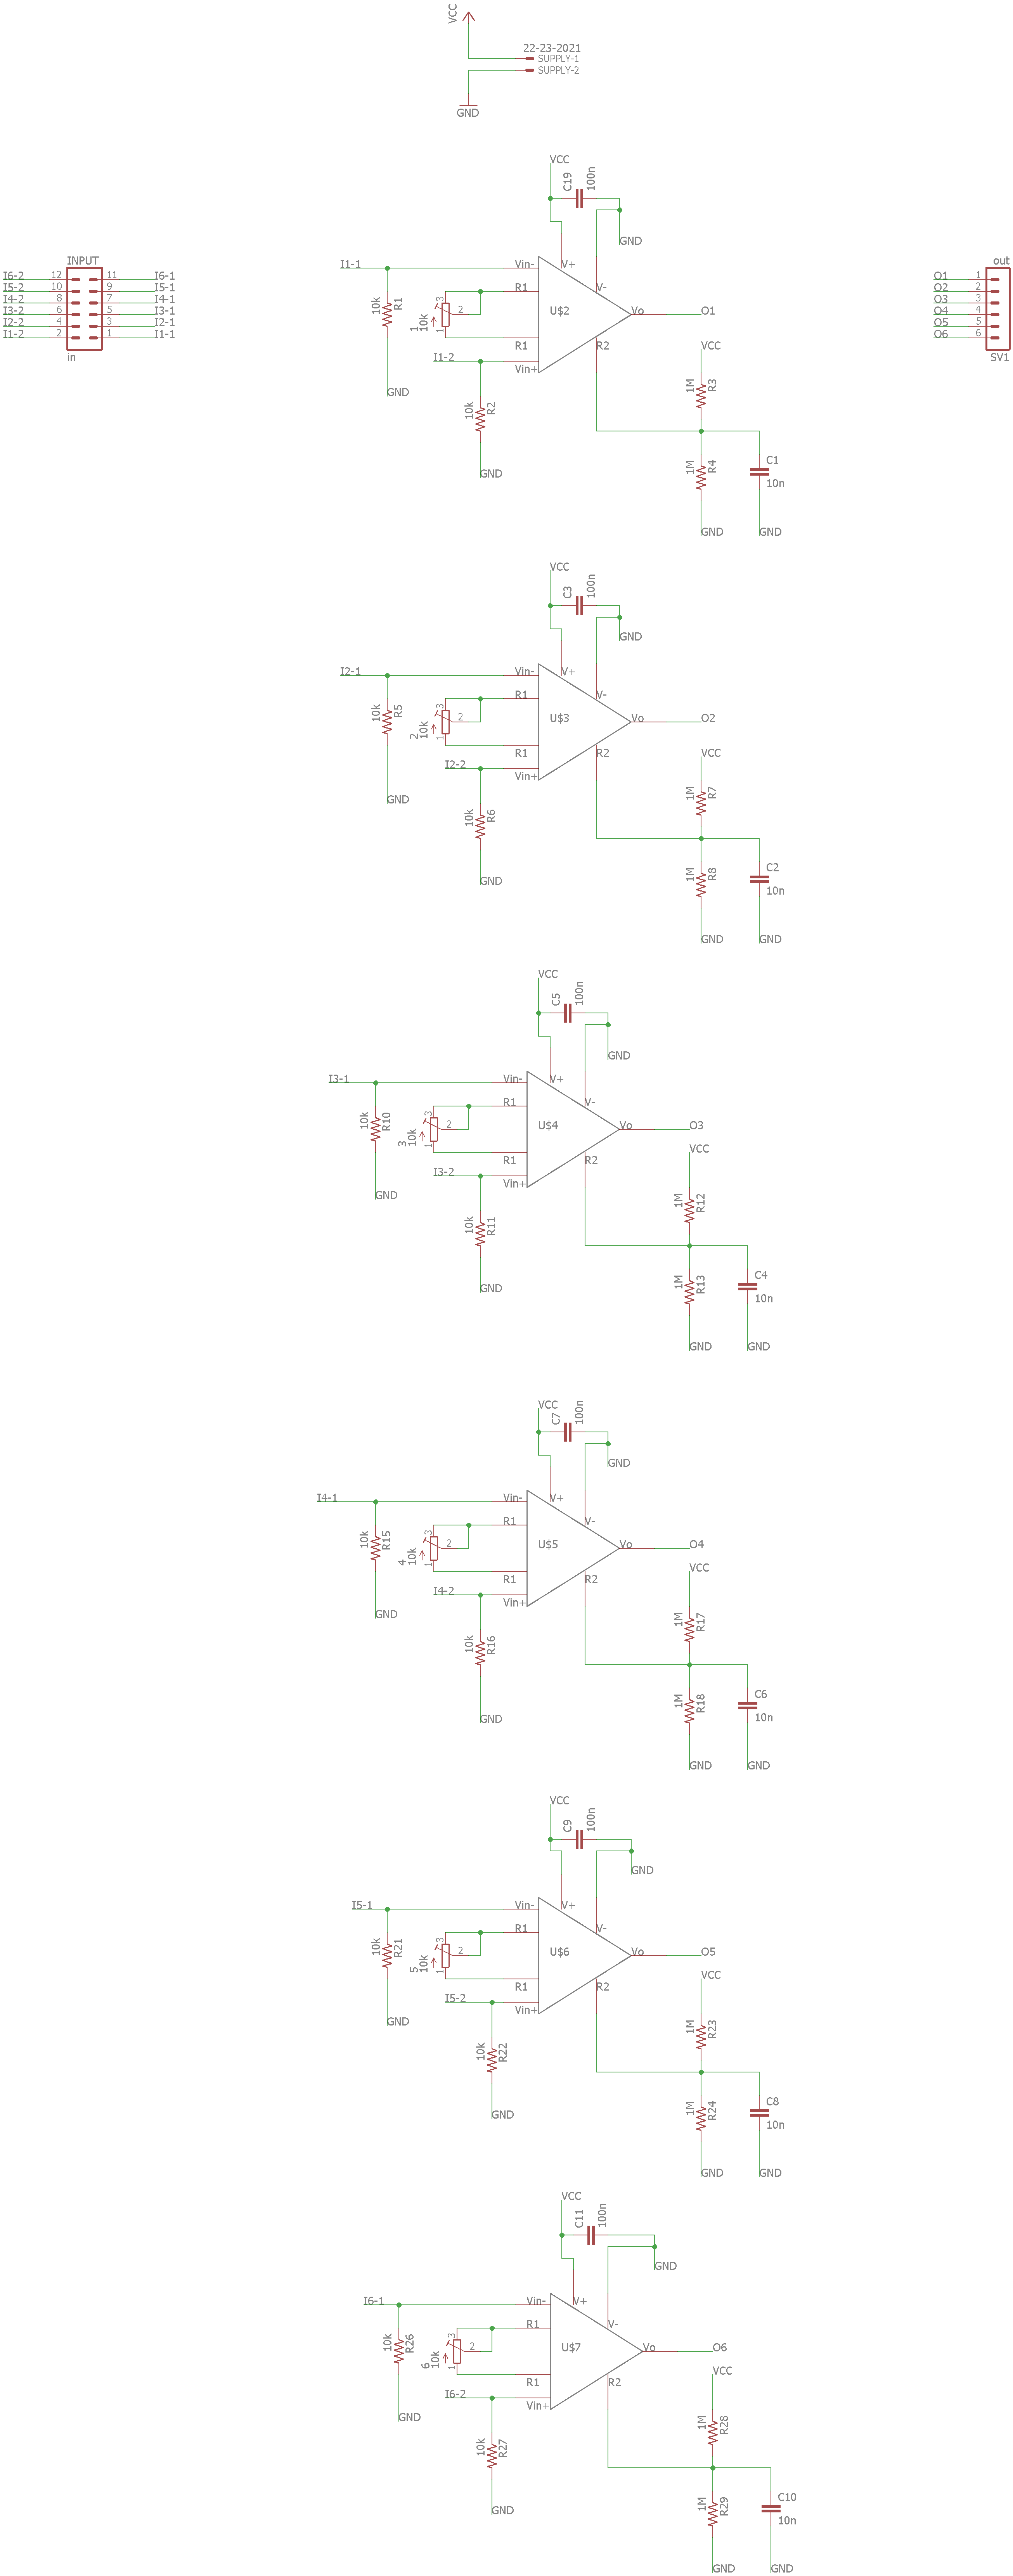
\includegraphics[scale=0.35]{images/INA/complete-schematic}
  \legend{Source: authors}
\end{figure}

\end{annexesenv}

\chapter{Prototype Cost Table.}

Costs are given on Brazilian Real.\\
\begin{table}[htb]
  \begin{center}
    \ABNTEXreducedfont
    \caption[Prototype Board Cost Table]{Prototype Board Cost Table}
    \label{Prototype-cost}
    \begin{tabular}{|c|c|c|}
      \hline
    Component & Quantity & Cost \\ \hline
    INA326 & 6 & 120.00\\ \hline
    10k$\Omega$ Trimmer Potentiometer & 6 & 7.50 \\ \hline
    10nF Ceramic Capacitor & 6 & 1.00 \\ \hline
    100nF Electrolytic Capacitor & 6 & 1.50 \\ \hline
    10k$\Omega$ Resistor 5$\%$ tolerancy & 12 & 2.00 \\ \hline
    1M$\Omega$ Resistor 5$\%$ tolerancy & 12 & 2.00 \\ \hline
    Pin bar 1x40 & 1 & 3.00 \\ \hline
    PCB & 2 & 50.00 \\ \hline
  \end{tabular}
  \legend{Source: authors}
\end{center}
\end{table}

\chapter{Production Cost Table.}

Costs are given on United States Dollar.\\
\begin{table}[htb]
  \begin{center}
    \ABNTEXreducedfont
    \caption[Production Board Prediction Cost Table]{Production Board Prediction Cost Table}
    \label{Production-cost}
    \begin{tabular}{|c|c|c|c|}
      \hline
    Component & Quantity & Cost per Component & Total Cost \\ \hline
    INA326 & 1000 & 2.53071 & 2530.71\\ \hline
    10k$\Omega$ Trimmer Potentiometer & 1000 & 0.64750 & 647.50 \\ \hline
    10nF Ceramic Capacitor & 1000 & 0.00278 & 2.78 \\ \hline
    100nF Electrolytic Capacitor & 1000 & 0.05861 & 58.61 \\ \hline
    10k$\Omega$ Resistor 1$\%$ tolerancy & 1000 & 0.01014 & 10.42 \\ \hline
    1M$\Omega$ Resistor 1$\%$ tolerancy & 1000 & 0.01078 & 10.78 \\ \hline
    Pin bar 1x40 & 1000 & 0.62240 & 622.40 \\ \hline
    PCB & 1000 & 0.22 & 223.94 \\ \hline
  \end{tabular}
  \legend{Source: \citeonline{Digikey} and \citeonline{PCB-maker} }
\end{center}
\end{table}


% Remissive index
\phantompart
\printindex

\end{document}
